% ============================================================
%  Práctica 1 --- Identificación del Motor CC
%  Dpto. Ingeniería de Sistemas y Automática --- Univ. de Sevilla
%  Estilo: Beamer Shadow (basado en Presentacion_arduino_V2.tex)
% ============================================================
\documentclass{beamer}
\usetheme{Shadow}

\usepackage[utf8]{inputenc}
\usepackage[T1]{fontenc}
\usepackage[spanish,es-nodecimaldot]{babel}
\usepackage{graphicx}
\usepackage{amsmath,amssymb}
\usepackage{booktabs}
\usepackage{array}
\usepackage{xcolor}
\usepackage{siunitx}
\usepackage{listings}
\usepackage{ragged2e}
\usepackage{transparent}

% ---- Listings (código MATLAB) ----
\lstset{
  language=Matlab,
  basicstyle=\tiny\ttfamily,
  keywordstyle=\color{blue!80!black},
  commentstyle=\color{green!50!black}\itshape,
  stringstyle=\color{orange!80!black},
  frame=single,
  breaklines=true,
  xleftmargin=4pt, xrightmargin=4pt,
}

%%%%%%%%%%%%%%%%%%%%%%%%%%%%%%%%%%
\title[Universidad de Sevilla\hspace{18mm}\insertframenumber/\inserttotalframenumber]{%
  Práctica 1 --- Identificación del Motor CC}
\institute{Dpto.\ de Ingeniería de Sistemas y Automática \\
           Escuela Superior de Ingenieros --- Universidad de Sevilla}
\date{}
%%%%%%%%%%%%%%%%%%%%%%%%%%%%%%%%%%

\xdefinecolor{isablue}{RGB}{0,70,130}
\xdefinecolor{isared}{RGB}{180,30,30}

%%%%%%%%%%%%%%%%%%%%%%%%%%%%%%%%%%
%     Custom headline (igual que referencia)
%%%%%%%%%%%%%%%%%%%%%%%%%%%%%%%%%%
\makeatletter
\setbeamertemplate{headline}{%
  \leavevmode%
  \@tempdimb=1.25ex%
  \ifnum\beamer@subsectionmax<\beamer@sectionmax%
    \multiply\@tempdimb by\beamer@sectionmax%
  \else%
    \multiply\@tempdimb by\beamer@subsectionmax%
  \fi%
  \ifdim\@tempdimb>0pt%
    \advance\@tempdimb by 1.125ex%
    \begin{beamercolorbox}[wd=.5\paperwidth,ht=\@tempdimb,right,rightskip=1em]%
        {section in head/foot}%
      \vbox to \@tempdimb{\vfill\insertsectionhead\vfill}%
    \end{beamercolorbox}%
    \begin{beamercolorbox}[wd=.5\paperwidth,ht=\@tempdimb]{subsection in head/foot}%
      \vbox to \@tempdimb{\vfill\insertsubsectionhead\vfill}%
    \end{beamercolorbox}%
  \fi%
}
\makeatother

%===========================================================
\begin{document}
%===========================================================

\begin{frame}
\titlepage
\end{frame}

\begin{frame}{Índice}
\tableofcontents
\end{frame}

%%%%%%%%%%%%%%%%%%%%%%%%%%%%%%%%%%
\section{Introducción al sistema}
%%%%%%%%%%%%%%%%%%%%%%%%%%%%%%%%%%

\subsection{El equipo ISA}

\begin{frame}{El equipo ISA}
El equipo de prácticas ha sido diseñado íntegramente por el Dpto.\ ISA.
Integra en una placa compacta (\textit{shield}) sobre Arduino~UNO
todos los elementos para controlar un motor CC real desde MATLAB/Simulink.
\begin{figure}[h]
  \centering
  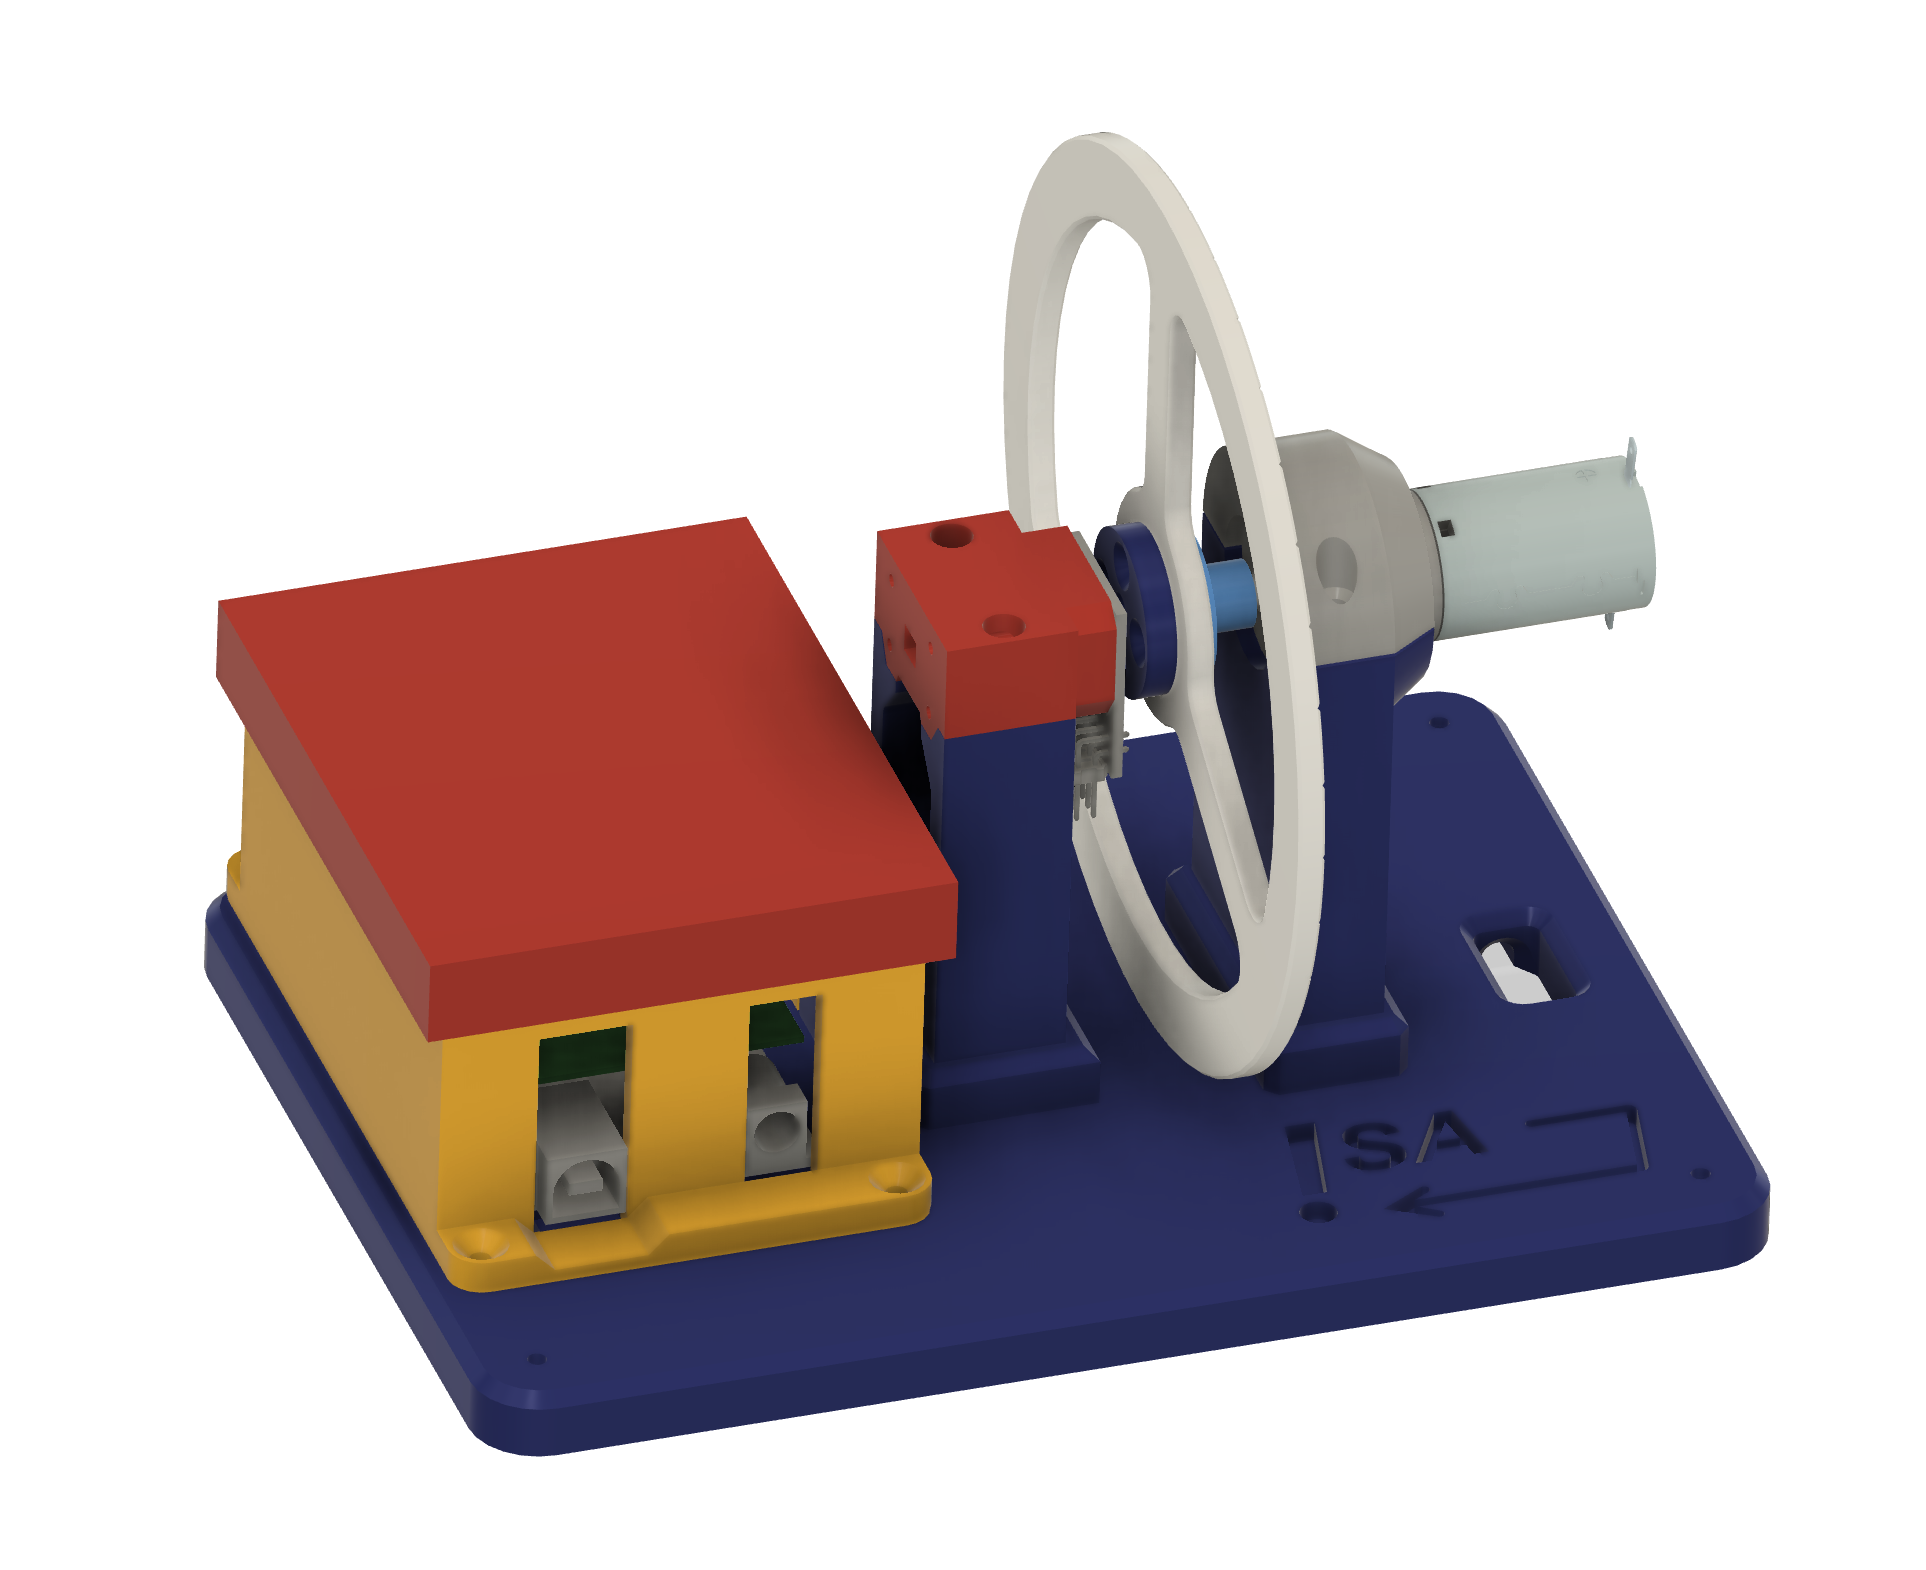
\includegraphics[width=6.5cm]{../../docs/images/equipo_render.png}
\end{figure}
\end{frame}

\begin{frame}{Componentes del equipo}
\begin{columns}[T]
  \column{0.52\textwidth}
  \begin{itemize}
    \item \textbf{Motor CC:} Maxon A-max~22, 5\,W, 12\,V con reductora GP~22B.
    \item \textbf{Encoder:} AS5047P, 14\,bits ($16\,384$ pasos/vuelta), magnético.
    \item \textbf{Driver:} TB6612FNG (puente en H dual). $u\in[-255,\,255]$.
    \item \textbf{Arduino UNO:} lee encoder (SPI), genera PWM, comunica con PC.
    \item \textbf{PC con MATLAB/Simulink:} ejecuta el controlador en tiempo real.
  \end{itemize}
  \column{0.45\textwidth}
  \begin{figure}[h]
    \centering
    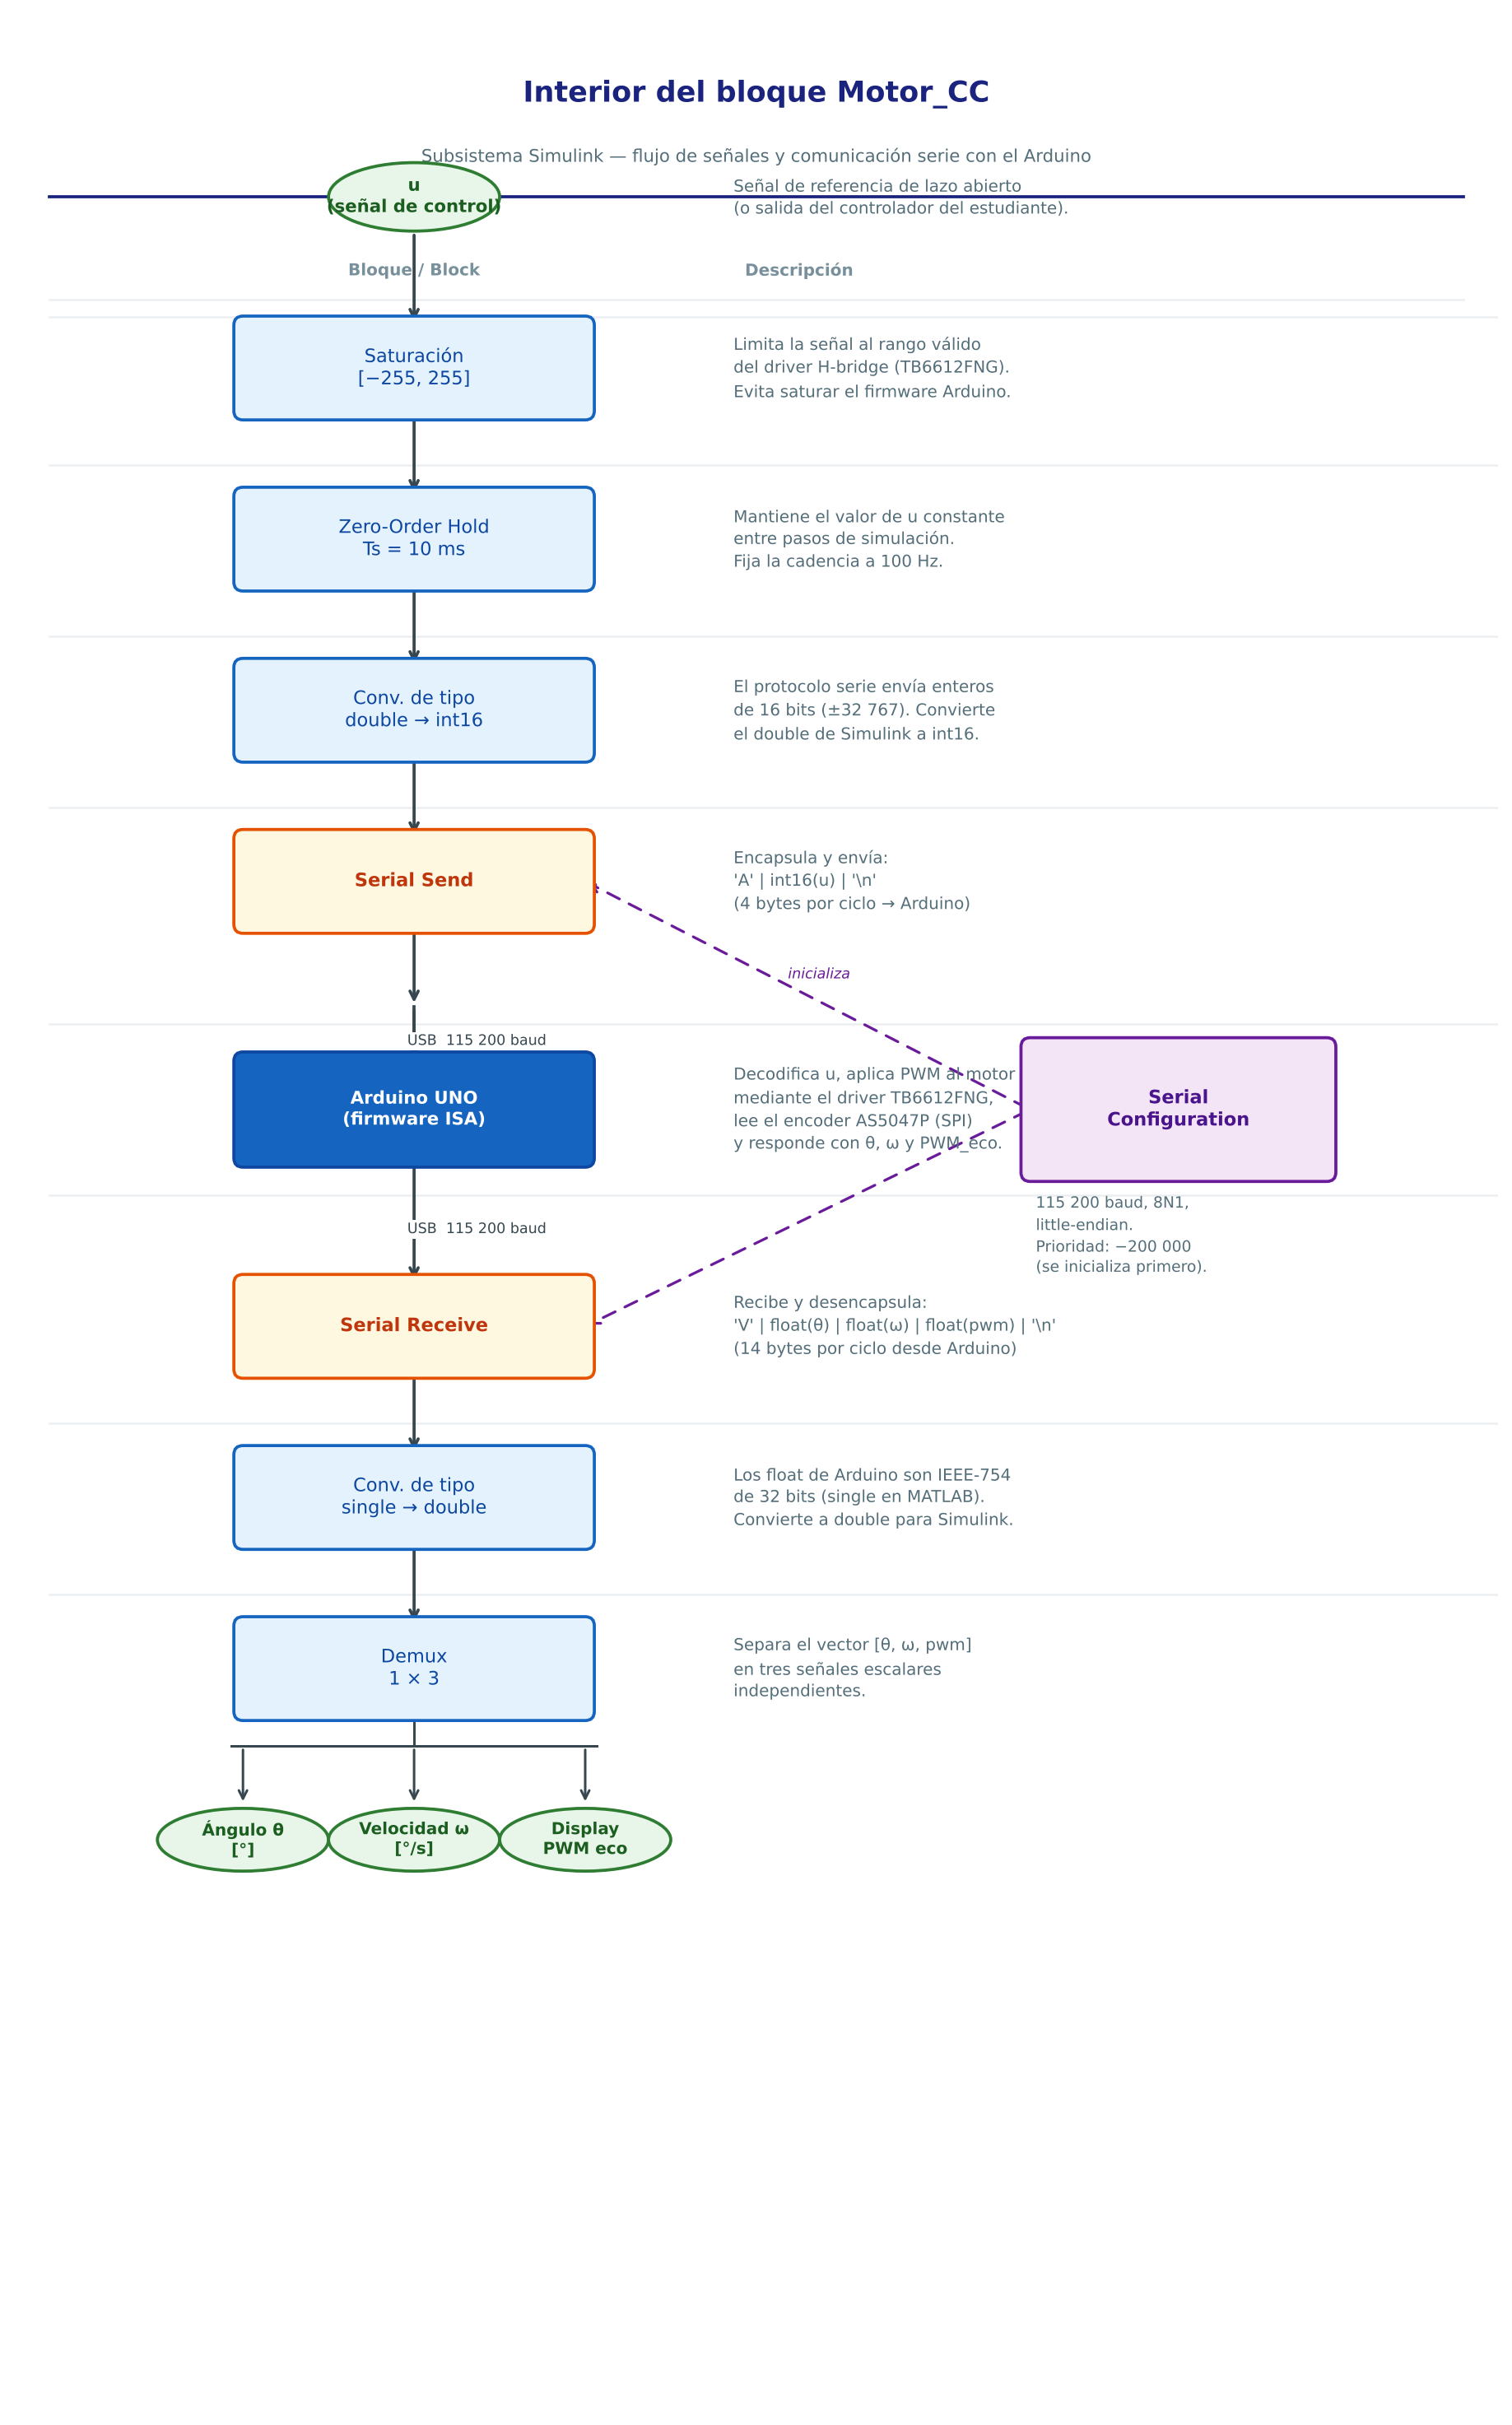
\includegraphics[width=\linewidth]{../../docs/images/matlab/diagram_motor_cc_es.png}
  \end{figure}
\end{columns}
\end{frame}

\subsection{Modelo matemático}

\begin{frame}{Modelo del motor CC}
El conjunto motor+reductora se modela como un sistema de \textbf{primer orden}:
\begin{block}{Función de transferencia}
\[
  G(s) = \frac{\Omega(s)}{V_{eq}(s)} = \frac{K}{\tau s + 1}
\]
\end{block}
\vspace{4pt}
\begin{columns}[T]
  \column{0.5\textwidth}
  \textbf{Parámetros a identificar:}
  \begin{itemize}
    \item $K$ [°/s\,/\,V]: ganancia estática.
    \item $\tau$ [s]: constante de tiempo mecánica.
  \end{itemize}
  \column{0.5\textwidth}
  \textbf{Señal de control:}
  \[ V_{eq} = u \cdot \frac{12\,\text{V}}{255} \]
  $u\in[-255,\;255]$ es el entero que envía Simulink.
\end{columns}
\vspace{6pt}
\textbf{Objetivo de la Práctica~1:} estimar $K$ y $\tau$ mediante ensayos
de escalón en lazo abierto.
\end{frame}

\subsection{Interfaz Simulink}

\begin{frame}{El bloque Motor\_CC}
Toda la comunicación con el Arduino está encapsulada en el bloque
\texttt{Motor\_CC} del modelo \texttt{MotorCC\_V3.slx}.
\vspace{6pt}
\begin{block}{Señales del bloque}
\begin{tabular}{lll}
\toprule
\textbf{Dirección} & \textbf{Señal} & \textbf{Descripción} \\
\midrule
Simulink $\to$ Arduino & $u$ & Control $[-255,\;255]$ \\
Arduino $\to$ Simulink & $\theta$ [°] & Posición angular acumulada \\
Arduino $\to$ Simulink & $\omega$ [°/s] & Velocidad angular \\
\bottomrule
\end{tabular}
\end{block}
\vspace{4pt}
\begin{itemize}
  \item Período de muestreo: $T_s = 10\,\text{ms}$ (100\,Hz).
  \item $u>0$ $\Rightarrow$ un sentido de giro;\quad $u<0$ $\Rightarrow$ sentido contrario;\quad $u=0$ $\Rightarrow$ parado.
\end{itemize}
\end{frame}

%%%%%%%%%%%%%%%%%%%%%%%%%%%%%%%%%%
\section{Laboratorio virtual con Simulink}
%%%%%%%%%%%%%%%%%%%%%%%%%%%%%%%%%%

\subsection{Simulación vs.\ lab. virtual}

\begin{frame}{Simulación vs.\ laboratorio virtual}
\begin{columns}[T]
  \column{0.48\textwidth}
  \begin{block}{Simulación clásica}
    \begin{itemize}
      \item Tiempo determinado (inicial--final).
      \item Entradas predefinidas.
      \item Análisis \emph{a posteriori}.
    \end{itemize}
  \end{block}
  \column{0.48\textwidth}
  \begin{block}{Laboratorio real/virtual}
    \begin{itemize}
      \item Stop Time = \texttt{Inf}.
      \item Modificación manual de $u$ en tiempo real.
      \item Visualización inmediata.
    \end{itemize}
  \end{block}
\end{columns}
\vspace{8pt}
\begin{alertblock}{En esta práctica}
  El modelo Simulink se comunica con el Arduino a 100\,Hz.
  Podemos cambiar $u$ mientras el motor está en marcha y ver la respuesta
  al instante.
\end{alertblock}
\end{frame}

\subsection{Configuración}

\begin{frame}{Configuración de la simulación}
Para trabajar en modo \emph{tiempo real interactivo}:
\begin{enumerate}
  \item Establezca \textbf{Stop Time} = \texttt{Inf}.
  \item \texttt{Run} $\to$ flecha desplegable $\to$ \emph{Simulation Pacing}.
  \item Active \emph{Enable pacing to slow down simulation}.
  \item Escoja \textbf{1\,s simulado / 1\,s real}.
\end{enumerate}
\begin{block}{Nota}
  Con el equipo real, la sincronía la fija el Arduino (100\,Hz); el
  \emph{pacing} evita que Simulink adelante los cálculos.
\end{block}
\end{frame}

\subsection{Controles de entrada}

\begin{frame}{Controles de entrada --- Dashboard}
Los bloques \texttt{Simulink / Dashboard} permiten modificar parámetros
de cualquier bloque \emph{sin detener la simulación}:
\begin{columns}[T]
  \column{0.45\textwidth}
  \textbf{Controles disponibles:}
  \begin{itemize}
    \item \textbf{Knob} --- dial giratorio.
    \item \textbf{Edit} --- campo de texto numérico.
    \item \textbf{Slider} --- deslizador.
  \end{itemize}
  \vspace{4pt}
  \textbf{Cómo conectar:}
  \begin{enumerate}\small
    \item Doble clic sobre el control.
    \item Seleccionar el bloque destino.
    \item Elegir el parámetro de la lista.
  \end{enumerate}
  \column{0.52\textwidth}
  \textbf{Uso en esta práctica:}
  \begin{itemize}
    \item \textbf{Knob} o \textbf{Edit} conectado al bloque \texttt{Constant}
          para fijar $u$.
    \item \texttt{Manual Switch} para conmutar entre constante y senoidal.
  \end{itemize}
\end{columns}
\end{frame}

\subsection{Indicadores de salida}

\begin{frame}{Scope y Dashboard Scope}
\begin{columns}[T]
  \column{0.48\textwidth}
  \begin{block}{Scope (Sinks)}
    \begin{itemize}
      \item \texttt{View $\to$ Configuration}:
        \begin{itemize}\small
          \item \textit{Time span}: no usar \texttt{Auto}.
          \item \textit{Update mode}: Wrap o Scroll.
          \item \textit{Y-Axis}: fijar mín. y máx.
        \end{itemize}
    \end{itemize}
  \end{block}
  \column{0.48\textwidth}
  \begin{block}{Dashboard Scope}
    \begin{itemize}
      \item Se incrusta dentro del diagrama.
      \item Doble clic $\to$ seleccionar señal.
      \item Ideal para supervisar $\theta$ y $\omega$ a la vez.
    \end{itemize}
  \end{block}
\end{columns}
\vspace{6pt}
\begin{block}{Data Inspector}
  \texttt{Simulation $\to$ Data Inspector}: registra todas las señales
  para análisis posterior. Dar nombre a cada señal y activar el icono de
  registro (\emph{log}).
\end{block}
\end{frame}

%%%%%%%%%%%%%%%%%%%%%%%%%%%%%%%%%%
\section{Puesta en marcha}
%%%%%%%%%%%%%%%%%%%%%%%%%%%%%%%%%%

\subsection{Pasos de puesta en marcha}

\begin{frame}{Puesta en marcha del equipo}
\begin{enumerate}
  \item \textbf{Conecte el Arduino} al PC por USB. Compruebe el LED de 12\,V.
  \item \textbf{Abra MATLAB} y navegue a \texttt{software/matlab/}.
  \item \textbf{Abra el modelo:} doble clic en \texttt{MotorCC\_V3.slx}.
  \item \textbf{Seleccione el puerto serie:}
        doble clic en el bloque \texttt{Motor\_CC} $\to$ desplegable
        \emph{Puerto serie} $\to$ seleccione el puerto del Arduino $\to$ \textbf{OK}.
  \item \textbf{Pulse Run} ($\triangleright$). La simulación arranca en tiempo real.
  \item \textbf{Verifique:} el Scope debe mostrar $\theta$ y $\omega$ actualizándose.
\end{enumerate}
\end{frame}

\subsection{Verificación}

\begin{frame}{Verificación del equipo}
Con el modelo en marcha:
\begin{enumerate}
  \item Fije $u = 50$ en el bloque \texttt{Constant}. El motor debe girar;
        $\theta$ sube (rampa), $\omega \approx \text{cte.}$
  \item Cambie a $u = -50$: el motor gira en sentido contrario.
  \item Fije $u = 0$: el motor se detiene.
  \item Configure Stop Time = \texttt{Inf} y pacing 1:1 para los experimentos.
\end{enumerate}
\begin{alertblock}{Si el motor no responde}
  \begin{itemize}
    \item Verifique el puerto serie en el bloque \texttt{Motor\_CC}.
    \item Compruebe que la fuente de 12\,V está encendida.
    \item Stop $\to$ Run (reinicio del modelo).
  \end{itemize}
\end{alertblock}
\end{frame}

%%%%%%%%%%%%%%%%%%%%%%%%%%%%%%%%%%
\section{Experimentos}
%%%%%%%%%%%%%%%%%%%%%%%%%%%%%%%%%%

\subsection{Ejercicio previo}

\begin{frame}{Ejercicio 1 --- Preguntas y script de inicialización}
\begin{block}{Preguntas teóricas}
  \begin{enumerate}
    \item ¿Cuál es la \textbf{entrada} del sistema motor CC?
    \item ¿Cuáles son las \textbf{salidas} medidas?
    \item ¿Qué ocurre si $|u| > 255$?
  \end{enumerate}
\end{block}
\vspace{4pt}
\begin{block}{Script \texttt{init\_motor.m}}
  \begin{lstlisting}
% init_motor.m --- Parámetros del equipo ISA Motor CC
u_max  = 255;   % Valor máximo de la señal de control
u_min  = -255;  % Valor mínimo de la señal de control
Ts     = 0.01;  % Periodo de muestreo [s]
V_alim = 12;    % Tensión de alimentación [V]
\end{lstlisting}
\end{block}
\end{frame}

\subsection{Experimento 1 --- Saturación}

\begin{frame}{Experimento 1 --- Efecto de la saturación en $u$}
\begin{block}{Procedimiento}
  Cambie $u$ progresivamente a través de los valores:
  \[ u \in \{-300,\;-255,\;-128,\;0,\;128,\;255,\;300\} \]
  Espere unos segundos en cada valor para que $\omega$ se estabilice.
\end{block}
\vspace{4pt}
Grafique $u$ y $\omega$ en un Scope con dos paneles y haga captura de pantalla.
\begin{alertblock}{Efecto de saturación en $u$}
  ¿Cambia $\omega$ al pasar de $u=255$ a $u=300$?
  ¿Y de $u=-255$ a $u=-300$?
\end{alertblock}
\end{frame}

\begin{frame}{Experimento 1 --- Gráfica y tabla}
\begin{center}
  \textit{[Pegue aquí la captura del Scope]}\\[2ex]
  \begin{tabular}{|c|c|}
    \hline
    $u$ & $\omega_{\infty}$ [°/s] \\ \hline
    $-255$ & \\ $-128$ & \\ $0$ & \\ $128$ & \\ $255$ & \\ \hline
  \end{tabular}
\end{center}
\end{frame}

\subsection{Experimento 2 --- Característica estática}

\begin{frame}{Experimento 2 --- Característica estática}
\begin{block}{Procedimiento}
  Mida $\omega_\infty$ en régimen permanente para:
  \[ u \in \{-255,\;-200,\;-128,\;-64,\;0,\;64,\;128,\;200,\;255\} \]
\end{block}
\begin{block}{Script MATLAB}
  \begin{lstlisting}
u_vec = [-255,-200,-128,-64, 0, 64,128,200,255];
w_vec = [   ?,   ?,   ?,  ?, ?,  ?,  ?,  ?,  ?]; % rellenar
plot(u_vec, w_vec, 'o-', 'LineWidth', 1.5)
xlabel('Señal de control u  [-]')
ylabel('\omega_\infty  [°/s]')
grid on;  title('Característica estática del motor CC')
\end{lstlisting}
\end{block}
\end{frame}

\begin{frame}{Experimento 2 --- Gráfica y preguntas}
\begin{center}
  \textit{[Pegue aquí la gráfica de la característica estática]}
\end{center}
\vspace{4pt}
\begin{block}{Preguntas}
  \begin{enumerate}
    \item ¿Es la relación $u \to \omega_\infty$ lineal? ¿Existe zona muerta?
    \item Estime la ganancia estática en la zona lineal:
          $K \approx \Delta\omega_\infty / \Delta V_{eq}$ [°/s\,/\,V].
  \end{enumerate}
\end{block}
\end{frame}

\subsection{Experimento 3 --- Ensayo en escalón}

\begin{frame}{Experimento 3 --- Ensayo en escalón}
\begin{block}{Procedimiento}
  \begin{enumerate}
    \item Parta de $u = 0$ con el motor parado.
    \item Aplique un escalón a $u = 128$ ($\approx 6$\,V).
    \item Espere hasta que $\omega$ alcance el régimen permanente ($\approx 5\tau$).
    \item Repita con $u = 200$ y $u = -128$.
  \end{enumerate}
\end{block}
Grafique $u$ (panel superior) y $\omega$ (panel inferior).
Haga captura de pantalla de cada ensayo.
\end{frame}

\begin{frame}{Experimento 3 --- Identificación de $K$ y $\tau$}
\begin{columns}[T]
  \column{0.5\textwidth}
  \begin{block}{Ganancia $K$}
    \[ K = \frac{\omega_\infty}{V_{eq}} = \frac{\omega_\infty}{u \cdot 12/255} \]
  \end{block}
  \vspace{4pt}
  \begin{block}{Constante de tiempo $\tau$}
    Tiempo en que $\omega$ alcanza el \textbf{63,2\,\%}
    de su valor final, medido desde el escalón.
  \end{block}
  \column{0.47\textwidth}
  \begin{tabular}{|l|c|}
    \hline
    \textbf{Magnitud} & \textbf{Valor} \\ \hline
    $u$ [−] & \\ $V_{eq}$ [V] & \\
    $\omega_\infty$ [°/s] & \\
    $K$ [°/s\,/\,V] & \\ $\tau$ [s] & \\ \hline
  \end{tabular}
\end{columns}
\end{frame}

\begin{frame}{Experimento 3 --- Gráfica y validación}
\begin{center}
  \textit{[Pegue aquí la captura del Scope --- respuesta al escalón]}
\end{center}
\vspace{4pt}
\begin{block}{Validación con MATLAB}
  \begin{lstlisting}
K = ?;  tau = ?;          % valores identificados
s = tf('s');
G = K / (tau*s + 1);
u0 = 128 * 12/255;        % tensión equivalente
step(u0*G)
hold on
% superponga los datos experimentales del Data Inspector
\end{lstlisting}
\end{block}
\end{frame}

\subsection{Experimento 4 --- Barrido frecuencial}

\begin{frame}{Experimento 4 --- Barrido de frecuencia (opcional)}
\begin{block}{Procedimiento}
  \begin{enumerate}
    \item Conecte $u$ a una señal senoidal: amplitud $A = 100$, bias $= 0$.
    \item Comience con $f = 0{,}1$\,Hz y aumente: 0,2 --- 0,5 --- 1 --- 2 --- 5\,Hz.
    \item Observe en el Scope la amplitud de $\omega$ en cada frecuencia.
  \end{enumerate}
\end{block}
\begin{block}{Pregunta}
  ¿A partir de qué frecuencia cae la amplitud de $\omega$?
  Compare con la frecuencia de corte teórica
  $f_c = 1/(2\pi\tau)$.
\end{block}
\end{frame}

%%%%%%%%%%%%%%%%%%%%%%%%%%%%%%%%%%
\section{Resumen}
%%%%%%%%%%%%%%%%%%%%%%%%%%%%%%%%%%

\begin{frame}{Resumen de la práctica}
\begin{block}{Resultados esperados}
  \begin{enumerate}
    \item \textbf{Característica estática:} gráfica $u$ vs.\ $\omega_\infty$.
    \item \textbf{Respuesta al escalón:} capturas del Scope (mínimo dos escalones).
    \item \textbf{Parámetros identificados:} $K$ [°/s\,/\,V] y $\tau$ [s].
    \item \textbf{Función de transferencia:} $G(s) = K/(\tau s+1)$ validada.
  \end{enumerate}
\end{block}
\vspace{4pt}
\begin{block}{Próximas prácticas}
  \begin{itemize}
    \item \textbf{Práctica 2:} diseño de un regulador PID.
    \item \textbf{Práctica 3:} control por realimentación de estados.
  \end{itemize}
\end{block}
\end{frame}

\end{document}
